{


\newcommand{\tnodeempty}{%
\begin{tikzpicture}[scale=0.3, baseline=(current bounding box.center)]
\useasboundingbox (0,-3) rectangle (3,3);
			\draw[thick, rounded corners=3pt] (0,0) rectangle (3,3);
			\draw[pattern=north west lines, pattern color=lightgray]  (3,0) to[rounded corners=3pt] (0,0) to[rounded corners=3pt] (0,3) to[rounded corners=3pt] (3,3) to[rounded corners=3pt] cycle;
;
			    \end{tikzpicture}
}

\newcommand{\todesingle}[1]{%
\begin{tikzpicture}[scale=0.3, baseline=(current bounding box.center)]
\useasboundingbox (0,-3) rectangle (3,3);
			\draw[thick, rounded corners=3pt] (0,0) rectangle (3,3);
			\node at (1.5, 1.5) {#1};
;
			    \end{tikzpicture}
}
\newcommand{\tone}{%
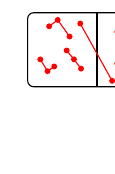
\begin{tikzpicture}[scale=0.25, every node/.style={scale=0.25}, baseline=(current bounding box.center)]
\useasboundingbox (0,-3) rectangle (3,3);
\def\xscale{1} % Horizontal scale factor
\def\yscale{1} % Vertical scale factor
\def\spnt{0.15} % Size of smaller points
\def\lpnt{0.125} % Size of larger points
\draw (3.52*\xscale, 3.76*\yscale) -- (3.52*\xscale, 0);
\draw[rounded corners=2ex*0.25] (0,0) rectangle (7.04*\xscale,3.76*\yscale);
\fill[red] (4.55*\xscale, 1.18*\yscale) circle (\spnt);
\fill[red] (6.05*\xscale, 2.78*\yscale) circle (\spnt);
\draw[red] (4.55*\xscale, 1.18*\yscale) -- (6.05*\xscale,2.78*\yscale);
\fill[red] (4.55*\xscale, 2.79*\yscale) circle (\spnt);
\fill[red] (6.05*\xscale, 1.12*\yscale) circle (\spnt);
\draw[red] (4.55*\xscale, 2.79*\yscale) -- (6.05*\xscale,1.12*\yscale);
\fill[red] (2.67*\xscale, 3.21*\yscale) circle (\spnt);
\fill[red] (4.29*\xscale, 0.3*\yscale) circle (\spnt);
\draw[red] (2.67*\xscale, 3.21*\yscale) -- (4.29*\xscale,0.3*\yscale);
\fill[red] (1.09*\xscale, 3.07*\yscale) circle (\spnt);
\fill[red] (1.526001050877835*\xscale, 3.393088634545991*\yscale) circle (\spnt);
\fill[red] (2.13*\xscale, 2.55*\yscale) circle (\spnt);
\draw[red] (1.09*\xscale, 3.07*\yscale) -- (1.526001050877835*\xscale,3.393088634545991*\yscale) -- (2.13*\xscale,2.55*\yscale);
\fill[red] (0.64*\xscale, 1.39*\yscale) circle (\spnt);
\fill[red] (1.01*\xscale, 0.79*\yscale) circle (\spnt);
\fill[red] (1.35*\xscale, 1.03*\yscale) circle (\spnt);
\draw[red] (0.64*\xscale, 1.39*\yscale) -- (1.01*\xscale,0.79*\yscale) -- (1.35*\xscale,1.03*\yscale);
\fill[red] (1.98*\xscale, 1.84*\yscale) circle (\spnt);
\fill[red] (2.3511520552717013*\xscale, 1.3932029657051672*\yscale) circle (\spnt);
\fill[red] (2.71*\xscale, 0.92*\yscale) circle (\spnt);
\draw[red] (1.98*\xscale, 1.84*\yscale) -- (2.3511520552717013*\xscale,1.3932029657051672*\yscale) -- (2.71*\xscale,0.92*\yscale);
\end{tikzpicture} 
}
\newcommand{\ttwo}{%
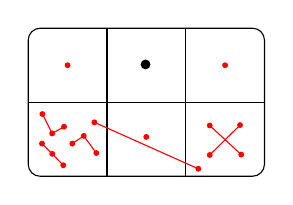
\begin{tikzpicture}[scale=0.5, every node/.style={scale=0.5}]
\def\xscale{1.0} % Horizontal scale factor
\def\yscale{1.0} % Vertical scale factor
\def\spnt{0.075} % Size of smaller points
\def\lpnt{0.125} % Size of larger points
\draw[rounded corners=2ex*0.5] (0,0) rectangle (6*\xscale,3.76*\yscale);
\draw (2.0*\xscale, 3.76*\yscale) -- (2.0*\xscale, 0);
\draw (4.0*\xscale, 3.76*\yscale) -- (4.0*\xscale, 0);
\draw (0, 1.88*\yscale) -- (6.0*\xscale, 1.88*\yscale);
\fill[red] (4.61*\xscale, 0.54*\yscale) circle (\spnt);
\fill[red] (5.38*\xscale, 1.3*\yscale) circle (\spnt);
\draw[red] (4.61*\xscale, 0.54*\yscale) -- (5.38*\xscale,1.3*\yscale);
\fill[red] (1.68*\xscale, 1.37*\yscale) circle (\spnt);
\fill[red] (4.32*\xscale, 0.19*\yscale) circle (\spnt);
\draw[red] (1.68*\xscale, 1.37*\yscale) -- (4.32*\xscale,0.19*\yscale);
\fill[red] (4.61*\xscale, 1.29*\yscale) circle (\spnt);
\fill[red] (5.41*\xscale, 0.55*\yscale) circle (\spnt);
\draw[red] (4.61*\xscale, 1.29*\yscale) -- (5.41*\xscale,0.55*\yscale);
\fill[red] (1.12*\xscale, 0.83*\yscale) circle (\spnt);
\fill[red] (1.4096601986560762*\xscale, 1.0249991174784614*\yscale) circle (\spnt);
\fill[red] (1.73*\xscale, 0.59*\yscale) circle (\spnt);
\draw[red] (1.12*\xscale, 0.83*\yscale) -- (1.4096601986560762*\xscale,1.0249991174784614*\yscale) -- (1.73*\xscale,0.59*\yscale);
\fill[red] (1*\xscale, 2.82*\yscale) circle (\spnt);
\fill[red] (5*\xscale, 2.82*\yscale) circle (\spnt);
\fill[red] (3*\xscale, 1*\yscale) circle (\spnt);
\fill[red] (0.36*\xscale, 1.58*\yscale) circle (\spnt);
\fill[red] (0.6091281492290661*\xscale, 1.0877096738635244*\yscale) circle (\spnt);
\fill[red] (0.91*\xscale, 1.26*\yscale) circle (\spnt);
\draw[red] (0.36*\xscale, 1.58*\yscale) -- (0.6091281492290661*\xscale,1.0877096738635244*\yscale) -- (0.91*\xscale,1.26*\yscale);
\fill[red] (0.35*\xscale, 0.83*\yscale) circle (\spnt);
\fill[red] (0.61*\xscale, 0.57*\yscale) circle (\spnt);
\fill[red] (0.89*\xscale, 0.28*\yscale) circle (\spnt);
\draw[red] (0.35*\xscale, 0.83*\yscale) -- (0.61*\xscale,0.57*\yscale) -- (0.89*\xscale,0.28*\yscale);
\fill (2.98*\xscale,2.84*\yscale) circle (\lpnt);
\end{tikzpicture}
}
\newcommand{\tthree}{%
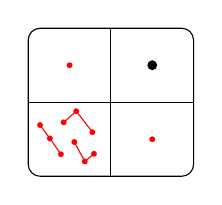
\begin{tikzpicture}[scale=0.5, every node/.style={scale=0.5}]
\def\xscale{1.0} % Horizontal scale factor
\def\yscale{1.0} % Vertical scale factor
\def\spnt{0.075} % Size of smaller points
\def\lpnt{0.125} % Size of larger points
\draw[rounded corners=2ex*0.5] (0,0) rectangle (4.2*\xscale,3.76*\yscale);
\draw (2.1*\xscale, 3.76*\yscale) -- (2.1*\xscale, 0);
\draw (0, 1.88*\yscale) -- (4.2*\xscale, 1.88*\yscale);
\fill[red] (1.05*\xscale, 2.82*\yscale) circle (\spnt);
\fill[red] (3.15*\xscale, 0.94*\yscale) circle (\spnt);
\fill[red] (0.9*\xscale, 1.37*\yscale) circle (\spnt);
\fill[red] (1.2199471753311761*\xscale, 1.6524363073940609*\yscale) circle (\spnt);
\fill[red] (1.63*\xscale, 1.12*\yscale) circle (\spnt);
\draw[red] (0.9*\xscale, 1.37*\yscale) -- (1.2199471753311761*\xscale,1.6524363073940609*\yscale) -- (1.63*\xscale,1.12*\yscale);
\fill[red] (1.17*\xscale, 0.87*\yscale) circle (\spnt);
\fill[red] (1.436829177631258*\xscale, 0.37686266458866924*\yscale) circle (\spnt);
\fill[red] (1.67*\xscale, 0.57*\yscale) circle (\spnt);
\draw[red] (1.17*\xscale, 0.87*\yscale) -- (1.436829177631258*\xscale,0.37686266458866924*\yscale) -- (1.67*\xscale,0.57*\yscale);
\fill[red] (0.3*\xscale, 1.3*\yscale) circle (\spnt);
\fill[red] (0.55*\xscale, 0.96*\yscale) circle (\spnt);
\fill[red] (0.83*\xscale, 0.56*\yscale) circle (\spnt);
\draw[red] (0.3*\xscale, 1.3*\yscale) -- (0.55*\xscale,0.96*\yscale) -- (0.83*\xscale,0.56*\yscale);
\fill (3.150000000000005*\xscale,2.8210223642172525*\yscale) circle (\lpnt);
\end{tikzpicture}
}
\newcommand{\tfour}{%
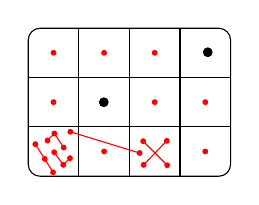
\begin{tikzpicture}[scale=0.5, every node/.style={scale=0.5}]
\def\xscale{1.0} % Horizontal scale factor
\def\yscale{1.0} % Vertical scale factor
\def\spnt{0.075} % Size of smaller points
\def\lpnt{0.125} % Size of larger points
\draw[rounded corners=2ex*0.5] (0,0) rectangle (5.14*\xscale,3.76*\yscale);
\draw (1.285*\xscale, 3.76*\yscale) -- (1.285*\xscale, 0);
\draw (2.57*\xscale, 3.76*\yscale) -- (2.57*\xscale, 0);
\draw (3.855*\xscale, 3.76*\yscale) -- (3.855*\xscale, 0);
\draw (0, 1.2533333333333332*\yscale) -- (5.14*\xscale, 1.2533333333333332*\yscale);
\draw (0, 2.5066666666666664*\yscale) -- (5.14*\xscale, 2.5066666666666664*\yscale);
\fill[red] ({(0*1.285+0.6425)*\xscale}, {(1*1.253+0.63)*\yscale}) circle (\spnt);
\fill[red] ({(0*1.285+0.6425)*\xscale}, {(2*1.253+0.63)*\yscale}) circle (\spnt);
\fill[red] ({(1*1.285+0.6425)*\xscale}, {(0*1.253+0.63)*\yscale}) circle (\spnt);
\fill[red] ({(1*1.285+0.6425)*\xscale}, {(2*1.253+0.63)*\yscale}) circle (\spnt);
\fill[red] ({(2*1.285+0.6425)*\xscale}, {(1*1.253+0.63)*\yscale}) circle (\spnt);
\fill[red] ({(2*1.285+0.6425)*\xscale}, {(2*1.253+0.63)*\yscale}) circle (\spnt);
\fill[red] ({(3*1.285+0.6425)*\xscale}, {(0*1.253+0.63)*\yscale}) circle (\spnt);
\fill[red] ({(3*1.285+0.6425)*\xscale}, {(1*1.253+0.63)*\yscale}) circle (\spnt);
\fill[red] (2.93*\xscale, 0.29*\yscale) circle (\spnt);
\fill[red] (3.52*\xscale, 0.9*\yscale) circle (\spnt);
\draw[red] (2.93*\xscale, 0.29*\yscale) -- (3.52*\xscale,0.9*\yscale);
\fill[red] (1.07*\xscale, 1.13*\yscale) circle (\spnt);
\fill[red] (2.83*\xscale, 0.59*\yscale) circle (\spnt);
\draw[red] (1.07*\xscale, 1.13*\yscale) -- (2.83*\xscale,0.59*\yscale);
\fill[red] (2.92*\xscale, 0.89*\yscale) circle (\spnt);
\fill[red] (3.53*\xscale, 0.28*\yscale) circle (\spnt);
\draw[red] (2.92*\xscale, 0.89*\yscale) -- (3.53*\xscale,0.28*\yscale);
\fill[red] (0.49*\xscale, 0.91*\yscale) circle (\spnt);
\fill[red] (0.6644210751853692*\xscale, 1.086774200246225*\yscale) circle (\spnt);
\fill[red] (0.9*\xscale, 0.73*\yscale) circle (\spnt);
\draw[red] (0.49*\xscale, 0.91*\yscale) -- (0.6644210751853692*\xscale,1.086774200246225*\yscale) -- (0.9*\xscale,0.73*\yscale);
\fill[red] (0.66*\xscale, 0.61*\yscale) circle (\spnt);
\fill[red] (0.89*\xscale, 0.29*\yscale) circle (\spnt);
\fill[red] (1.06*\xscale, 0.46*\yscale) circle (\spnt);
\draw[red] (0.66*\xscale, 0.61*\yscale) -- (0.89*\xscale,0.29*\yscale) -- (1.06*\xscale,0.46*\yscale);
\fill[red] (0.18033887520734232*\xscale, 0.816133743581277*\yscale) circle (\spnt);
\fill[red] (0.42*\xscale, 0.44*\yscale) circle (\spnt);
\fill[red] (0.63*\xscale, 0.1*\yscale) circle (\spnt);
\draw[red] (0.18033887520734232*\xscale, 0.816133743581277*\yscale) -- (0.42*\xscale,0.44*\yscale) -- (0.63*\xscale,0.1*\yscale);
\fill (1.92*\xscale,1.88*\yscale) circle (\lpnt);
\fill (4.56*\xscale,3.15*\yscale) circle (\lpnt);
\end{tikzpicture}
}
\newcommand{\tpair}{%
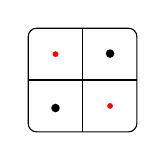
\begin{tikzpicture}[scale=0.35, every node/.style={scale=0.35}, baseline=(current bounding box.center)]
\def\xscale{1.0} % Horizontal scale factor
\def\yscale{1.0} % Vertical scale factor
\def\spnt{0.105} % Size of smaller points
\def\lpnt{0.155} % Size of larger points
\draw[rounded corners=2ex*.35] (0,0) rectangle (3.94*\xscale,3.76*\yscale);
\draw (1.97*\xscale, 3.76*\yscale) -- (1.97*\xscale, 0);
\draw (0, 1.88*\yscale) -- (3.94*\xscale, 1.88*\yscale);
\fill (0.99*\xscale,0.864920127795527*\yscale) circle (\lpnt);
\fill (2.97*\xscale,2.841054313099042*\yscale) circle (\lpnt);
\fill[red] (0.99*\xscale,3.76*0.75*\yscale) circle (\spnt);
\fill[red] (3*0.99*\xscale,3.76*0.25*\yscale) circle (\spnt);
\end{tikzpicture}
}
\begin{center}
\scalebox{1}{\begin{tikzpicture}
    \node (root) at (-0.5, 0) {\tone};
    \node (lvl_1_1) at (-3,-2.25) {\ttwo};
    \node (lvl_1_2) at (0,-2.25) {\tnodeempty};
    \node (lvl_1_3) at (3,-2.25) {\tthree};
    
    \node (lvl_2_1) at (-4.5,-5.5) {\tone};
    \node (lvl_2_2) at (-2, -5.5) {\todesingle{\point{0.08}}};
    
    \node (lvl_2_3) at (1.75,-5.5) {\tfour};
    \node (lvl_2_4) at (4.25,-5.5) {\todesingle{\point{0.08}}};
    
    \node (lvl_3_1) at (0,-9) {\tone};
    \node (lvl_3_2) at (3.25,-8.73) {\tpair};
    
    \node (lvl_4_1) at (2,-11.75) {\todesingle{\point{0.08}}};
    \node (lvl_4_2) at (4.5,-11.75) {\todesingle{\point{0.08}}};
    
    \ptedge{(root)}{(0,1.2)}{(lvl_1_1)}{(-0.5,1.3)}
    \ptedge{(root)}{(0,1.2)}{(lvl_1_2)}{(-0.5,1.3)}
    \ptedge{(root)}{(0,1.2)}{(lvl_1_3)}{(-0.5,1.3)}
    
    \ptedge{(lvl_1_1)}{(-0.5,0.25)}{(lvl_2_1)}{(0,1.3)}
    \ptedge{(lvl_1_1)}{(-0.5,0.25)}{(lvl_2_2)}{(-0.5,1.3)}
    \ptedge{(lvl_1_3)}{(-0.5,0.25)}{(lvl_2_3)}{(-0.5,1.3)}
    \ptedge{(lvl_1_3)}{(-0.5,0.25)}{(lvl_2_4)}{(-0.5,1.3)}
    
    \ptedge{(lvl_2_3)}{(-0.5,0.25)}{(lvl_3_1)}{(0,1.3)}
    \ptedge{(lvl_2_3)}{(-0.5,0.25)}{(lvl_3_2)}{(-0.5,1.02)}
    
    
    \ptedge{(lvl_3_2)}{(-0.5,0.53)}{(lvl_4_1)}{(-0.5,1.3)}
    \ptedge{(lvl_3_2)}{(-0.5,0.53)}{(lvl_4_2)}{(-0.5,1.3)}
\end{tikzpicture}}
\end{center}
}